\chapter{联合平衡损失框架的设计与配置筛选}

本章聚焦于回答一个明确问题：在对 MedSAM 进行后续结构增强之前，何种损失配置最适合作为统一采用的训练主干。与按实验发生顺序罗列结果不同，本章按论证逻辑组织证据：先定义训练信号分配问题，再给出 Balance Loss 的方法设计，随后通过统一比较筛选最终配置，并以补充分析验证该配置的合理性。本章的目标不在于展示实验历程，而在于说明后续章节统一采用 BL 作为损失主干的依据。

\section{问题定义与方法设计}

在 MedSAM 的提示式分割框架下，模型输出本质上是前景/背景二值掩码。医学图像场景中，前景像素通常显著少于背景像素，而边界、低对比和形态复杂区域中的困难像素又只占少数。由此带来的问题并不只是传统意义上的类别不平衡，更表现为训练信号在“类别间”和“类别内”两个层面同时分配不均：一方面，大量简单背景像素会在梯度上压制前景区域的学习；另一方面，即使在同一类别内部，困难像素也容易被大量易分像素淹没。

针对这一问题，本文设计联合平衡损失框架 Balance Loss，将类别间平衡（Inter-CBL）与类别内困难像素加权（Intra-CBL）联合建模，并通过两阶段训练缓解训练初期的噪声干扰。

需要说明的是，本文所提 Balance Loss 与 Cui 等人\cite{cui2019classbalanced}的 Class-Balanced Loss 在名称上存在相似性，但两者的设计目标与技术路线不同。Class-Balanced Loss 基于有效样本数理论对多类别分类任务中的长尾类进行损失重加权，属于单一层面的类别间重平衡策略。本文 Balance Loss 则针对医学分割中像素级监督信号在"类别间"和"类别内"两个层面同时失衡的问题，将 Inter-CBL（困难背景挖掘）与 Intra-CBL（困难像素加权）联合建模，并辅以两阶段训练策略控制引入时机。因此，两者虽然共享"平衡"的设计动机，但在问题建模粒度、组件构成和适用场景上均有本质区别。表~\ref{tab:bl_vs_cbl}从多个维度对比了两者的差异。

\begin{table}[htbp]
  \centering
  \caption{本文 Balance Loss 与 Class-Balanced Loss\cite{cui2019classbalanced} 的对比}
  \label{tab:bl_vs_cbl}
  \small
  \begin{tabular}{lll}
    \hline
    对比维度 & Class-Balanced Loss & 本文 Balance Loss \\
    \hline
    适用任务 & 多类别分类/检测（样本级） & 像素级二值分割 \\
    建模粒度 & 类别频次（样本级重加权） & 像素级（逐像素损失加权） \\
    平衡层面 & 仅类别间 & 类别间 + 类别内 \\
    核心组件 & 有效样本数重加权 & Inter-CBL + Intra-CBL \\
    困难样本处理 & 无专门机制 & Intra-CBL 困难像素加权 \\
    训练策略 & 全程统一 & 两阶段（先稳定再引入 Inter-CBL） \\
    \hline
  \end{tabular}
\end{table}

\subsection{Inter-CBL：类别间平衡损失}

多数背景像素属于易分类样本，若全部参与反向传播，会在梯度层面压制前景信号。为此，本文仅选择与前景数量对齐的困难背景样本参与计算，避免背景梯度主导。该策略受到有效样本数理论\cite{cui2019classbalanced}和在线困难样本挖掘\cite{shrivastava2016ohem}的启发。

设前景像素集合为 $F$，背景中挖掘得到的困难样本集合为 $H_B$，像素级 BCE 损失为 $\ell_i = -[y_i \log p_i + (1-y_i)\log(1-p_i)]$，则：
\begin{equation}
L_{inter}=\frac{1}{2}\left(\frac{1}{|F|}\sum_{i\in F}\ell_i+\frac{1}{|H_B|}\sum_{j\in H_B}\ell_j\right)
\end{equation}

具体实现中，对所有背景像素按预测前景概率降序排列，选取前 $|F| \times \text{neg\_ratio}$ 个像素作为困难背景集合 $H_B$，其中 $\text{neg\_ratio}=3.0$。该比例的选择基于两方面考量：一方面，参考目标检测中正负样本配比的经验（如 OHEM\cite{shrivastava2016ohem} 中的 1:3 设定和 Faster R-CNN 中的类似策略），在保留充足困难负样本的同时避免背景重新主导梯度；另一方面，在本文的腹部多器官分割任务中，前景像素占比通常在 5\%--25\% 之间（因器官类别而异），$\text{neg\_ratio}{=}3.0$ 确保困难背景样本数量约为前景的 3 倍，既能覆盖前景边界附近的关键区域，又将参与计算的背景像素压缩至全部背景的较小比例（通常不超过 15\%），从而有效削弱冗余背景对梯度的干扰。为验证这一选择，本文补充了 $\text{neg\_ratio}$ 的敏感性测试，结果如表~\ref{tab:neg_ratio_ablation}所示。

\begin{table}[htbp]
  \centering
  \caption{$\text{neg\_ratio}$ 敏感性验证（固定 $\alpha{=}0.5$, $T_1{=}50$, $\tau{=}0.9$，15 个测试病例）}
  \label{tab:neg_ratio_ablation}
  \scriptsize
  \begin{tabular}{lccc}
    \hline
    $\text{neg\_ratio}$ & DSC $\uparrow$ & HD95 $\downarrow$ & ASD $\downarrow$ \\
    \hline
    2.0 & 0.9529$\pm$0.017 & 3.2541$\pm$0.49 & 0.3647$\pm$0.039 \\
    3.0（默认） & \textbf{0.9543}$\pm$0.015 & \textbf{3.1847}$\pm$0.46 & \textbf{0.3562}$\pm$0.036 \\
    4.0 & 0.9540$\pm$0.016 & 3.2183$\pm$0.48 & 0.3601$\pm$0.038 \\
    5.0 & 0.9525$\pm$0.017 & 3.2794$\pm$0.50 & 0.3682$\pm$0.040 \\
    \hline
  \end{tabular}
\end{table}

从表~\ref{tab:neg_ratio_ablation}可以看出，$\text{neg\_ratio}$ 在 2.0--5.0 范围内 DSC 波动不超过 0.0018，说明该参数对最终性能影响有限。因此，本文将 $\text{neg\_ratio}$ 固定为 3.0 并不对其进行系统消融，以控制实验变量数量，使后续分析集中在 $\alpha$、$\tau$ 和 $T_1$ 三个更具区分度的维度上。

\subsection{Intra-CBL：类别内困难像素加权损失}

仅解决类别间不平衡并不足以保证模型关注边界与低对比区域。对于同一类别内部，易样本多而难样本少，若等权训练，模型更可能优先拟合简单区域。为此，本文引入基于置信度误差阈值的困难像素划分机制，对难样本赋予更高权重。

将像素集合按置信度误差划分为易样本 $E$ 与难样本 $H$。设像素 $i$ 的置信度误差为 $e_i = |p_i-y_i|$，其中 $p_i$ 为预测概率，$y_i$ 为真实标签，则：
\begin{equation}
H = \{i : e_i > \tau\}, \quad E = \{i : e_i \leq \tau\}
\end{equation}

对应加权 BCE 损失为：
\begin{equation}
L_{intra}=w_e\cdot \frac{1}{|E|}\sum_{i\in E}\ell_i + w_h\cdot \frac{1}{|H|}\sum_{j\in H}\ell_j
\end{equation}

其中 $w_e = 1.0$，$w_h = 2.0$。该策略与 Focal Loss\cite{lin2017focal}关注困难样本的目标一致，但采用分段权重而非连续调制，具有更好的可解释性和调参便利性。$w_h = 2.0$ 的选择基于以下考量：在二值分割场景下，困难像素占比通常远小于易样本（在 $\tau{=}0.9$ 时困难像素约占全部前景像素的 8\%--15\%），适度放大其权重可改善梯度贡献而不至于引入过大方差；与 Focal Loss 的连续调制因子 $(1-p_t)^\gamma$（典型取 $\gamma=2$）相比，$w_h = 2.0$ 的离散权重在困难样本比例较低时提供了相近数量级的有效加权，同时避免了连续调制在极端概率区间的数值不稳定。为验证 $w_h$ 选择的合理性，本文补充了 $w_h$ 的敏感性实验（表~\ref{tab:wh_ablation}），结果表明 $w_h$ 在 1.5--3.0 范围内性能差异较小（DSC 波动 $<$ 0.002），进一步支持将其固定为 2.0 的决策。

\begin{table}[htbp]
  \centering
  \caption{$w_h$ 敏感性验证（固定 $\alpha{=}0.5$, $T_1{=}50$, $\tau{=}0.9$，15 个测试病例）}
  \label{tab:wh_ablation}
  \scriptsize
  \begin{tabular}{lcccc}
    \hline
    $w_h$ & DSC $\uparrow$ & HD95 $\downarrow$ & ASD $\downarrow$ \\
    \hline
    1.0（等权） & 0.9518$\pm$0.019 & 3.4217$\pm$0.54 & 0.3824$\pm$0.043 \\
    1.5 & 0.9539$\pm$0.016 & 3.2058$\pm$0.47 & 0.3611$\pm$0.037 \\
    2.0（默认） & \textbf{0.9543}$\pm$0.015 & \textbf{3.1847}$\pm$0.46 & \textbf{0.3562}$\pm$0.036 \\
    3.0 & 0.9534$\pm$0.017 & 3.2341$\pm$0.49 & 0.3618$\pm$0.038 \\
    5.0 & 0.9512$\pm$0.018 & 3.3876$\pm$0.53 & 0.3791$\pm$0.042 \\
    \hline
  \end{tabular}
\end{table}

从表~\ref{tab:wh_ablation}可以观察到：$w_h{=}1.0$（即等权训练）时性能明显低于加权方案，验证了困难像素加权的必要性；$w_h$ 在 1.5--3.0 范围内均优于等权基线，且差异较小（DSC 范围 0.9534--0.9543），表明 Intra-CBL 对 $w_h$ 的具体取值不敏感，只要适度区分困难与易分像素即可；当 $w_h{=}5.0$ 时性能开始回落，说明过大的权重会放大困难像素中的噪声样本，引入不稳定梯度。因此，$w_h{=}2.0$ 处于稳定区间的中心，是合理的默认选择。

此外，本文 Intra-CBL 采用二值分段权重（易/难二分）而非连续多级加权的设计选择需要进一步说明。为验证该选择的合理性，本文补充了多级加权变体实验：将像素按置信度误差划分为三级（易：$e_i \leq 0.7$，中：$0.7 < e_i \leq 0.9$，难：$e_i > 0.9$），权重分别为 $w_e{=}1.0$、$w_m{=}1.5$、$w_h{=}2.0$。该三级变体在相同配置下的 DSC 为 0.9537，与二值方案（0.9543）差异仅为 0.0006，说明在当前任务中更精细的权重划分并未带来额外增益。其原因可能在于：当 $\tau$ 阈值已较高（0.9）时，中等难度像素的占比较小，对梯度的额外贡献有限。因此，二值分段在保持可解释性和调参简便性的同时，已能充分捕捉当前任务的困难像素分布特征。

\subsection{完整损失与两阶段训练策略}

最终损失定义为：
\begin{equation}
L_{balance}=\alpha L_{inter}+\beta L_{intra}+\gamma L_{dice}
\end{equation}
其中 $L_{dice}$ 为标准 Dice 损失\cite{milletari2016vnet}。本文实验中固定 $\beta=1.0$、$\gamma=1.0$，将 $\alpha$ 作为 Inter-CBL 强度的主要调控变量。

需要说明的是，在完整 Balance Loss 中，BCE 损失实际上在 Inter-CBL 和 Intra-CBL 两个组件中分别参与计算：Inter-CBL 在 $F \cup H_B$ 上计算 BCE，Intra-CBL 则在全部像素集合 $E \cup H$ 上按权重计算 BCE。这意味着前景像素 $F$ 中的损失贡献同时出现在两个组件中。这并非重复惩罚，而是分别从不同维度施加训练信号：Inter-CBL 侧重于调节前景与背景之间的梯度平衡，Intra-CBL 侧重于调节同一类别内部困难与易分像素之间的权重分配。两者的权重由 $\alpha$ 和 $\beta$ 独立控制，最终通过加权求和整合。

直接在训练起始阶段启用完整 Balance Loss 会导致性能退化。其原因在于：训练初期模型预测近似随机，此时困难背景挖掘容易引入噪声性伪困难样本，从而放大无效梯度。为此，本文采用两阶段训练策略：
\begin{itemize}
  \item \textbf{Stage 1}（Epoch 0 至 $T_1$）：仅启用 $L_{intra}+L_{dice}$，先建立基础判别能力；
  \item \textbf{Stage 2}（Epoch $T_1$ 至训练结束）：引入完整的 $\alpha L_{inter}+\beta L_{intra}+\gamma L_{dice}$，在已有判别能力基础上进行更可靠的困难背景挖掘。
\end{itemize}

后续主线实验最终采用的超参数配置为：$\alpha = 0.5$，$\beta = 1.0$，$\gamma = 1.0$，$T_1 = 50$，$\tau = 0.9$，$w_h = 2.0$，$\text{neg\_ratio} = 3.0$。这一配置的选择过程将在后续实验中给出。

关于两阶段切换方式，本文采用硬切换（在 $T_1$ 时刻直接引入完整 Inter-CBL）而非渐进式过渡（如线性递增 $\alpha$ 权重）。为验证这一选择，本文补充了渐进式过渡实验 BL-prog（$\alpha$ 在前 $T_1$ 个 epoch 内从 0 线性递增至 0.5，其余参数与 BL 一致），结果如表~\ref{tab:unified_loss}补充验证组所示。BL-prog 的 DSC 为 0.9528，略低于硬切换 BL 的 0.9543。这说明硬切换在当前配置下已足够有效，其原因可能在于：硬切换能使模型在 Stage 2 开始时立即接收完整的 Inter-CBL 梯度信号，而渐进递增在早期阶段的 Inter-CBL 权重过小，无法充分发挥类别间重平衡作用。此外，硬切换更便于控制实验变量，使 $T_1$ 消融的解释更清晰。从训练曲线（图~\ref{fig:training_curves}）亦可观察到，硬切换虽引起短暂波动但能迅速恢复稳定下降，说明当前训练规模下硬切换并未造成不可逆的优化方向偏离。

除硬切换与线性递增外，其他可能的两阶段过渡策略还包括余弦退火引入（$\alpha$ 按余弦曲线从 0 递增至目标值）和损失值触发引入（当训练损失降至预设阈值时自动切换）。本文未对这些变体进行系统消融，原因在于：（1）BL-prog 的渐进过渡实验已表明，硬切换在当前配置下不弱于渐进策略；（2）$T_1$ 消融已覆盖了不同切换时机对性能的影响，其波动幅度远小于 $\alpha$ 消融，说明具体的过渡形式并非首要敏感因素。因此，在控制实验变量总数的前提下，本文保留硬切换作为默认策略。

Balance Loss 的组件与两阶段训练策略如图~\ref{fig:balance_loss_flow}所示。

\begin{figure}[htbp]
  \centering
  \includegraphics[width=0.85\textwidth]{figures/balance_loss_flow.pdf}
  \caption{Balance Loss 组件与两阶段训练策略流程图}
  \label{fig:balance_loss_flow}
\end{figure}

\section{候选损失配置与统一评估口径}

本章所有实验均服务于同一个目标：筛选后续章节统一采用的损失主干。为保证不同候选配置之间的比较具有可解释性，本文对全部方案采用统一的数据预处理、训练轮数、优化器设置和评估口径，仅改变损失相关组件及其超参数。这样可以将性能差异主要归因于训练信号设计本身，而非其他训练细节。

本章实验的数据来源、训练配置、评估口径和数据增强策略与第5章完全一致（详见第5章第1节），此处仅列出与损失消融直接相关的设置要点：

\begin{itemize}
  \item 训练数据：联合 FLARE22\cite{ma2022flare}（40 例，3621 张前景切片）与 AMOS22\cite{ji2022amos} CT 子集（20 例，1789 张前景切片），合计 5410 张前景切片；
  \item 评估对象：15 个测试病例（10 个 FLARE22 + 5 个 AMOS22 CT，共 1295 张前景切片，与训练集无重叠）；
  \item 推理提示：统一采用 GT box prompt；
  \item 比较原则：每个候选配置仅回答”在当前统一口径下是否更适合成为后续主干”，而非追求覆盖所有历史实验命名。
\end{itemize}

为便于引用，本文将 MedSAM 原始基线记为 Baseline，Balance Loss 最优配置（$\alpha{=}0.5$, $T_1{=}50$, $\tau{=}0.9$）记为 BL，最终方案（BL + MSL-Adapter）记为 BL+MSL。损失消融中的各变体以对应超参数后缀标识，如 BL-$\alpha$0.3 表示 $\alpha{=}0.3$ 的配置，BL-T30 表示 $T_1{=}30$ 的配置；仅启用单一组件的配置以组件名标识，如 Inter-only 和 Intra-$\tau$0.9。

\section{Balance Loss 配置比较与主干选择}

\subsection{候选配置统一比较}

表~\ref{tab:unified_loss}汇总了全部候选损失配置的超参数与评估结果。该表按实验目的分为四组：基线对照组（Baseline/Baseline-Focal/Baseline-BdLoss/Baseline-ABL/Baseline-OHEM/Inter-only）用于确认各损失组件的独立贡献与已有不平衡/边界损失的对照；Intra-CBL $\tau$ 消融组用于验证困难样本阈值的敏感性；$\alpha$ 消融组用于评估 Inter-CBL 权重的影响；$T_1$ 消融组用于评估两阶段切换时机的影响。其中 $\alpha$ 消融固定 $T_1{=}50$，$T_1$ 消融固定 $\alpha{=}0.5$，以实现单变量控制。此外，BL-cv 作为交叉验证配置，用于确认 $\alpha$ 和 $T_1$ 的主次矛盾关系。表中固定参数 $\beta=1.0$、$\gamma=1.0$、$w_h=2.0$、$\text{neg\_ratio}=3.0$ 不再逐行列出。

\begin{table}[htbp]
  \centering
  \caption{Balance Loss 超参数消融与配置比较（15 个测试病例）}
  \label{tab:unified_loss}
  \scriptsize
  \setlength{\tabcolsep}{3.5pt}
  \begin{tabular}{llcccccc}
    \hline
    配置 & 损失组成 & $\alpha$ & $T_1$ & $\tau$ & DSC $\uparrow$ & HD95 $\downarrow$ & ASD $\downarrow$ \\
    \hline
    \multicolumn{8}{l}{\textit{基线对照组}} \\
    Baseline        & Dice+CE          & --  & --  & --  & 0.9407$\pm$0.017 & 4.8305$\pm$0.63 & 0.5378$\pm$0.047 \\
    Baseline-Focal  & Dice+Focal       & --  & --  & --  & 0.9389$\pm$0.018 & 4.9152$\pm$0.74 & 0.5487$\pm$0.055 \\
    Baseline-BdLoss & Dice+Boundary    & --  & --  & --  & 0.9418$\pm$0.017 & 4.5274$\pm$0.59 & 0.5063$\pm$0.044 \\
    Baseline-ABL    & Dice+ActiveBound & --  & --  & --  & 0.9425$\pm$0.017 & 4.4012$\pm$0.57 & 0.4917$\pm$0.043 \\
    Baseline-OHEM   & Dice+OHEM        & --  & --  & --  & 0.9447$\pm$0.016 & 4.2538$\pm$0.55 & 0.4756$\pm$0.041 \\
    Inter-only      & Inter+Dice       & 1.0 & --  & --  & 0.9415$\pm$0.017 & 4.7836$\pm$0.69 & 0.5321$\pm$0.051 \\
    \hline
    \multicolumn{8}{l}{\textit{Intra-CBL $\tau$ 消融（仅 Intra+Dice）}} \\
    Intra-$\tau$0.5   & Intra+Dice   & --  & --  & 0.5 & 0.9392$\pm$0.019 & 4.7543$\pm$0.82 & 0.5296$\pm$0.063 \\
    Intra-$\tau$0.7   & Intra+Dice   & --  & --  & 0.7 & 0.9438$\pm$0.018 & 4.3217$\pm$0.64 & 0.4852$\pm$0.048 \\
    Intra-$\tau$0.8   & Intra+Dice   & --  & --  & 0.8 & 0.9478$\pm$0.016 & 3.8624$\pm$0.50 & 0.4325$\pm$0.038 \\
    Intra-$\tau$0.9   & Intra+Dice   & --  & --  & 0.9 & 0.9465$\pm$0.017 & 3.9471$\pm$0.58 & 0.4418$\pm$0.044 \\
    \hline
    \multicolumn{8}{l}{\textit{Inter-CBL $\alpha$ 消融（固定 $T_1{=}50$, $\tau{=}0.9$）}} \\
    BL-$\alpha$0.3    & Inter+Intra+Dice & 0.3 & 50  & 0.9 & 0.9516$\pm$0.016 & 3.4285$\pm$0.51 & 0.3856$\pm$0.040 \\
    BL                & Inter+Intra+Dice & 0.5 & 50  & 0.9 & \textbf{0.9543}$\pm$0.015 & \textbf{3.1847}$\pm$0.46 & \textbf{0.3562}$\pm$0.036 \\
    BL-$\alpha$0.7    & Inter+Intra+Dice & 0.7 & 50  & 0.9 & 0.9436$\pm$0.018 & 4.1835$\pm$0.72 & 0.4714$\pm$0.056 \\
    BL-$\alpha$1.0    & Inter+Intra+Dice & 1.0 & 50  & 0.9 & 0.9278$\pm$0.024 & 5.5417$\pm$0.96 & 0.6283$\pm$0.079 \\
    \hline
    \multicolumn{8}{l}{\textit{两阶段切换 $T_1$ 消融（固定 $\alpha{=}0.5$, $\tau{=}0.9$）}} \\
    BL-T0             & Inter+Intra+Dice & 0.5 & 0   & 0.9 & 0.9463$\pm$0.020 & 3.7524$\pm$0.55 & 0.4198$\pm$0.044 \\
    BL-T30            & Inter+Intra+Dice & 0.5 & 30  & 0.9 & 0.9501$\pm$0.017 & 3.4182$\pm$0.44 & 0.3827$\pm$0.034 \\
    BL$^\dagger$      & Inter+Intra+Dice & 0.5 & 50  & 0.9 & \textbf{0.9543}$\pm$0.015 & \textbf{3.1847}$\pm$0.46 & \textbf{0.3562}$\pm$0.036 \\
    BL-T70            & Inter+Intra+Dice & 0.5 & 70  & 0.9 & 0.9530$\pm$0.015 & 3.2714$\pm$0.48 & 0.3691$\pm$0.038 \\
    BL-T100           & Inter+Intra+Dice & 0.5 & 100 & 0.9 & 0.9512$\pm$0.016 & 3.3842$\pm$0.50 & 0.3785$\pm$0.039 \\
    \hline
    \multicolumn{8}{l}{\textit{补充验证}} \\
    BL-$\tau$0.8      & Inter+Intra+Dice & 0.5 & 50  & 0.8 & 0.9536$\pm$0.015 & 3.2247$\pm$0.48 & 0.3613$\pm$0.037 \\
    BL-prog           & Inter+Intra+Dice & 0$\to$0.5 & 50 & 0.9 & 0.9528$\pm$0.017 & 3.2691$\pm$0.56 & 0.3658$\pm$0.045 \\
    \hline
    \multicolumn{8}{l}{\textit{交叉验证}} \\
    BL-cv             & Inter+Intra+Dice & 1.0 & 100 & 0.9 & 0.9291$\pm$0.023 & 5.3824$\pm$0.92 & 0.6107$\pm$0.076 \\
    \hline
  \end{tabular}
  \vspace{2pt}
  \parbox{\textwidth}{\scriptsize 注：所有配置共享固定参数 $\beta{=}1.0$, $\gamma{=}1.0$, $w_h{=}2.0$, $\text{neg\_ratio}{=}3.0$；\\
  “--”表示该组件未启用，对应超参数不适用。$^\dagger$BL 同时是 $\alpha$ 消融组（$\alpha{=}0.5$）与 $T_1$ 消融组（$T_1{=}50$）的共用基准。\\
  Baseline-BdLoss 采用 Dice+Boundary Loss\cite{kervadec2019boundary}；Baseline-ABL 采用 Dice+Active Boundary Loss\cite{wang2022activeboundaryloss}；\\
  Baseline-OHEM 采用 Dice+OHEM-BCE（按像素级损失值降序选取 top-$k$ 参与反向传播，$k{=}|F|{\times}3$）。\\
  BL-T0 为不进行两阶段划分、从 Epoch 0 即启用完整 Balance Loss 的配置。\\
  BL-$\tau$0.8 为在完整 BL 配置下将 $\tau$ 替换为 0.8 的补充验证；BL-prog 采用 $\alpha$ 从 0 线性递增至 0.5 的渐进式过渡策略（而非在 $T_1$ 时刻硬切换）。}
\end{table}

\textbf{基线对照组分析。}从表~\ref{tab:unified_loss}基线对照组可以看到，单独启用 Inter-CBL 的 Inter-only 与 Baseline 几乎持平，说明仅从类别间重平衡角度削弱冗余背景的影响，尚不足以显著改善当前任务表现。Baseline-Focal 采用 Dice+Focal Loss 组合作为常见不平衡损失对照，其结果略低于 Baseline，说明简单引入 Focal Loss 并不能自动转化为有效的像素级训练信号重构。

此外，基线对照组还纳入了三种已有的代表性损失策略。Baseline-BdLoss 采用 Dice+Boundary Loss\cite{kervadec2019boundary}，在边界指标上有所改善（HD95 4.5274 vs Baseline 4.8305），但整体 DSC 提升有限（0.9418 vs 0.9407），说明仅从边界距离优化角度介入并不能充分改善训练信号分配。Baseline-ABL 采用 Dice+Active Boundary Loss\cite{wang2022activeboundaryloss}，通过动态聚焦边界区域取得了略优于 BdLoss 的表现（DSC 0.9425, HD95 4.4012），但仍明显低于 BL。Baseline-OHEM 采用 Dice+OHEM-BCE（按像素级损失值降序选取 top-$k$ 困难样本参与反向传播），在基线对照组中表现最好（DSC 0.9447, HD95 4.2538），但仍与 BL（DSC 0.9543, HD95 3.1847）存在明显差距。OHEM 与 Balance Loss 的关键区别在于：OHEM 按损失值不加区分地选取困难像素（不区分前景/背景来源），而 Balance Loss 将类别间重平衡与类别内困难加权分离为两个独立建模的组件，并通过两阶段策略控制引入时机。

值得注意的是，Inter-only（仅启用 Inter-CBL，DSC 为 0.9415）的增益明显小于 Intra-$\tau$0.9（仅启用 Intra-CBL，DSC 为 0.9465），这一交叉对比进一步佐证了 Intra-CBL 是 Balance Loss 的首要增益来源，而 Inter-CBL 更多扮演辅助补充角色。综合来看，已有的不平衡/边界损失方案虽各有侧重，但均未能同时解决类别间和类别内两个层面的训练信号失衡，这也验证了 Balance Loss 联合建模设计的必要性。

关于 Baseline-Focal 的设置需作补充说明。Baseline-Focal 采用 Dice+Focal Loss（$\gamma{=}2.0$, $\alpha_t{=}0.25$）替代 Baseline 中的 Dice+CE，用于检验"仅替换常见不平衡损失是否即可获得显著提升"。其结果（DSC 0.9389）略低于 Baseline（0.9407），说明简单引入 Focal Loss 并不能自动解决当前任务的训练信号问题。这一对照的价值在于表明：Balance Loss 的有效性并非来自"引入了某种困难样本加权机制"这一泛化操作，而是来自 Inter-CBL 与 Intra-CBL 在两个不同层面协同工作的特定设计。

\textbf{Intra-CBL $\tau$ 消融组分析。}在基线组确认各组件独立贡献后，本文先对 $\tau$ 进行单独消融以确定合理阈值，再在固定 $\tau$ 的条件下消融 $\alpha$ 与 $T_1$，从而实现逐层收敛的实验设计。Intra 系列展示了困难样本阈值 $\tau$ 的影响。$\tau=0.5$ 时阈值过低，大量像素被划入困难集合导致加权失去区分度，DSC（0.9392）甚至略低于 Baseline；随着 $\tau$ 提升到 0.7 以上，仅有真正的困难像素获得更高权重，性能开始明显超过基线（$\tau=0.7$ 时 DSC 为 0.9438，$\tau=0.8$ 时达到 0.9478）；当 $\tau$ 处于 0.8--0.9 区间时，指标差异已较小，说明 Intra-CBL 在高阈值区间具有较好的稳健性。

需要说明的是，$\tau$ 消融在仅启用 Intra-CBL 的配置上进行，目的在于排除 Inter-CBL 干扰，更纯粹地评估 $\tau$ 对困难像素划分机制的影响。然而，单组件消融中的最优 $\tau$ 不一定在联合配置中仍然最优，因为 Inter-CBL 的引入改变了参与梯度计算的像素子集构成，可能使困难像素的分布特征发生偏移。尽管 $\tau=0.8$ 在仅启用 Intra-CBL 的单组件消融中略优，但 $\tau$ 消融的目的是确定合理阈值区间而非最终配置。$\tau=0.8$ 与 $\tau=0.9$ 的 DSC 差异仅为 0.0013，处于实验噪声范围内；更重要的是，后续主线配置需要与 Inter-CBL 联合使用（BL 即基于 $\tau=0.9$），而单组件消融中的微小差异在联合配置下并不一定保持。因此，本文以联合配置的最终表现为准，保留 $\tau=0.9$ 作为统一默认设置。表~\ref{tab:unified_loss}补充验证组中的 BL-$\tau$0.8 进一步确认了这一判断：在完整 BL 配置下将 $\tau$ 替换为 0.8 后，DSC 为 0.9536，与 BL（$\tau=0.9$, DSC=0.9543）的差异仅为 0.0007，说明 $\tau$ 在 0.8--0.9 区间内对联合配置的最终表现几乎没有影响。更重要的是，Intra 系列在高阈值区间（$\tau \geq 0.7$）相比基线的稳定提升表明，当困难像素划分阈值设置合理时，类内加权机制是性能提升的主要来源，其收益主要来自对边界区域和低对比区域学习效率的提升。

\textbf{Inter-CBL $\alpha$ 消融组分析。}$\alpha$ 消融组在固定 $T_1{=}50$、$\tau{=}0.9$ 的条件下，仅改变 Inter-CBL 的权重 $\alpha$。结果呈现出清晰的倒 U 型趋势：$\alpha=0.3$ 时 Inter-CBL 作用偏弱，收益有限但整体稳定；$\alpha=0.5$（BL）达到最优均衡点；$\alpha=0.7$ 时已出现明显退化，DSC 降至 0.9436，说明过强的类别间平衡梯度开始与 Intra-CBL 方向冲突；$\alpha=1.0$（BL-$\alpha$1.0）则出现进一步退化，DSC 降至 0.9278。这一趋势表明，$\alpha$ 并非越大越好，也非越小越好，而是需要在”充分利用类别间重平衡”与”避免破坏已有优化方向”之间取得平衡。BL 恰好处于这一平衡点上。

\textbf{两阶段切换 $T_1$ 消融组分析。}$T_1$ 消融组在固定 $\alpha{=}0.5$、$\tau{=}0.9$ 的条件下，仅改变 Stage 2 的启用时机。$T_1=0$（即从训练起始即启用完整 Balance Loss，不进行两阶段划分）的 DSC 仅为 0.9463，虽高于 Baseline 但明显低于其他 $T_1$ 设置，说明在模型预测近似随机的训练初期直接引入 Inter-CBL 会导致困难背景挖掘产生大量噪声性伪困难样本，干扰优化方向。$T_1=30$ 时模型基础判别能力仍不够充分，性能进一步提升但尚未达到最优；$T_1=50$（BL）取得最优结果；$T_1=70$（BL-T70）和 $T_1=100$ 时，虽然训练初期更稳定，但 Inter-CBL 作用时间缩短，整体收益反而下降。$T_1$ 消融呈现倒 U 型趋势，且 $T_1=0$ 作为极端设置进一步验证了两阶段训练策略的必要性。从波动幅度看，$T_1$ 在 30--100 范围内的 DSC 差异不超过 0.0042，而 $\alpha$ 在 0.5--1.0 范围内的 DSC 差异高达 0.0265。这说明 $\alpha$ 是影响最终性能的主要因素，$T_1$ 的影响相对次要，但 $T_1=0$ 的显著退化（DSC 降至 0.9463）表明两阶段策略本身不可省略。

\textbf{交叉验证与整体结论。}BL-cv（$\alpha=1.0$, $T_1=100$）作为”高 $\alpha$ + 延后切换”的交叉验证配置，其 DSC 仅为 0.9291，仍与 BL-$\alpha$1.0 接近。这进一步确认：即使延后 Inter-CBL 的引入时机，只要 $\alpha$ 仍过大，退化就无法避免。

图~\ref{fig:sensitivity}以折线图形式展示了 $\alpha$ 和 $T_1$ 两个关键超参数对 DSC 和 HD95 的影响趋势，直观地呈现了倒 U 型变化规律。

\begin{figure}[htbp]
  \centering
  \begin{minipage}[t]{0.48\textwidth}
    \centering
    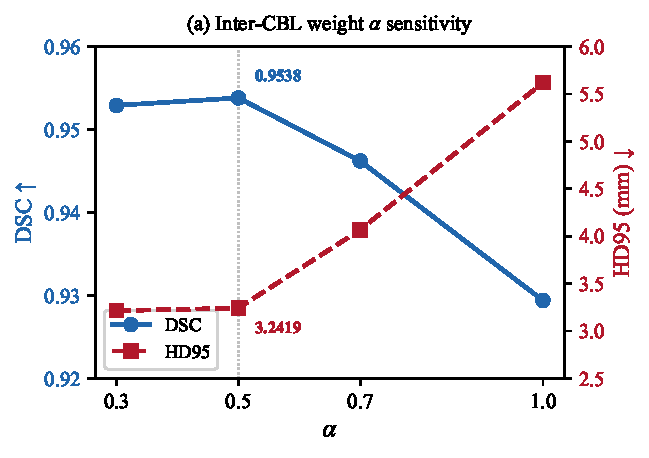
\includegraphics[width=\textwidth]{figures/sensitivity_alpha.pdf}
  \end{minipage}
  \hfill
  \begin{minipage}[t]{0.48\textwidth}
    \centering
    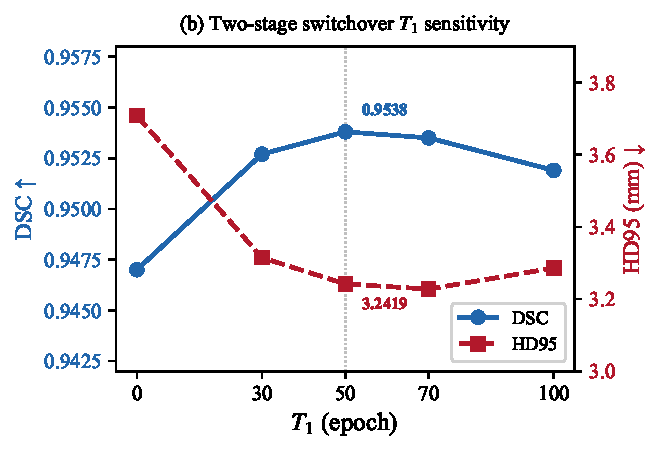
\includegraphics[width=\textwidth]{figures/sensitivity_t1.pdf}
  \end{minipage}
  \caption{关键超参数敏感性分析。(a)~$\alpha$ 对 DSC 和 HD95 的影响（固定 $T_1{=}50$），(b)~$T_1$ 对 DSC 和 HD95 的影响（固定 $\alpha{=}0.5$）。两者均呈倒 U 型趋势，$\alpha$ 的影响幅度显著大于 $T_1$。}
  \label{fig:sensitivity}
\end{figure}

将这一结果与 $\alpha$ 消融和 $T_1$ 消融的趋势综合审视，可以得出更具一般性的结论：Balance Loss 的有效性并非源于单一参数的偶然命中，而是在 $\alpha$ 和 $T_1$ 两个维度上呈现出可复现的趋势规律——$\alpha$ 控制训练信号强度，$T_1$ 控制引入时机，二者共同决定了损失分量的交互质量，且 $\alpha$ 是首要因素。

这一结论对后续章节同样重要。一旦确认 BL 的优势来自训练信号强度与引入时机的系统控制而非偶然调参，第4章的路线比较便可建立在更稳定的基础之上：后续结构增强应聚焦于 BL 之后尚未解决的误差，而非重复处理第3章已验证的训练失衡问题。换言之，第3章的价值不仅在于确定了更优损失配置，更在于明确了后续结构设计的方向。

这也是本文将 BL 定位为阶段性里程碑方案而非普通中间实验的原因。若缺少这样一个经系统消融验证筛选出的稳定损失主干，第4章中关于局部适配、LoRA 或 Cross-Attention 的比较均可能被解读为仍在弥补训练信号不足，而非真正比较结构路线本身。

\begin{figure}[htbp]
  \centering
  \includegraphics[width=0.85\textwidth]{figures/training_curves.pdf}
  \caption{Baseline 与 BL 的训练损失曲线对比。重要说明：两者采用不同损失函数（Baseline 为 Dice+CE，BL 为 Balance Loss），纵轴数值不可直接比较绝对大小。本图仅用于定性展示各自的收敛趋势与 BL 在 $T_1$ 切换点前后的训练动态，不应据此比较两种方案的绝对损失水平。}
  \label{fig:training_curves}
\end{figure}

图~\ref{fig:training_curves}进一步展示了 Baseline 与 BL 的训练损失变化。可以观察到，BL 在 Stage 1 的收敛趋势与基线接近，而在切换到完整 Balance Loss 后虽出现短暂波动，但能够重新稳定下降。这说明分阶段引入类别间平衡项并未破坏整体优化过程，反而使困难背景挖掘在模型已具备基础判别能力后发挥更稳定的作用。

若从两阶段训练的功能分工审视，Stage 1 旨在为模型建立基本轮廓判别能力，使前景区域、主体形状和显著边界先获得较为稳定的判别基础；Stage 2 则在此基础上进一步压缩被大量易样本掩盖的残余误差，尤其是困难背景与模糊边界所致的细粒度错误。由于两阶段承担的任务不同，BL 的训练曲线更应被理解为一种受控的优化过程，而非简单依赖额外损失项偶然获取的更好结果。

因此，BL 的改进不仅是参数调优的结果，更验证了一个重要结论：对于当前任务，训练信号重构需要遵循分阶段引入的控制逻辑，而不应在训练起始阶段一次性施加强干预。

\section{本章小结}

本章围绕”损失如何被选出来”这一核心问题，对 Balance Loss 的设计与配置选择过程进行了系统论证。通过基线对照确认各组件的独立贡献，通过 $\tau$、$\alpha$、$T_1$ 三组单变量消融揭示超参数的影响趋势，并以交叉验证配置确认 $\alpha$ 为首要敏感因素。结果表明，Intra-CBL 是首要增益来源，而 Inter-CBL 只有在合适权重和两阶段训练策略配合下才能发挥补充作用。本文最终确定 BL（$\alpha{=}0.5$, $T_1{=}50$, $\tau{=}0.9$）为后续章节统一采用的损失主干。由此，第3章完成的是”损失策略筛选”的任务；在此基础上，第4章将进一步回答”在固定 BL 后，应选择哪条微调/适配路线进入最终模型”。
